%%%%%%%%%%%%%%%%%%%%%%% file typeinst.tex %%%%%%%%%%%%%%%%%%%%%%%%%
%
% This is the LaTeX source for the instructions to authors using
% the LaTeX document class 'llncs.cls' for contributions to
% the Lecture Notes in Computer Sciences series.
% http://www.springer.com/lncs       Springer Heidelberg 2006/05/04
%
% It may be used as a template for your own input - copy it
% to a new file with a new name and use it as the basis
% for your article.
%
% NB: the document class 'llncs' has its own and detailed documentation, see
% ftp://ftp.springer.de/data/pubftp/pub/tex/latex/llncs/latex2e/llncsdoc.pdf
%
%%%%%%%%%%%%%%%%%%%%%%%%%%%%%%%%%%%%%%%%%%%%%%%%%%%%%%%%%%%%%%%%%%%


\documentclass[runningheads,a4paper]{llncs}

\usepackage{amssymb}
\setcounter{tocdepth}{3}
\usepackage{graphicx}
\usepackage{hyperref}
\usepackage{amsmath}
\usepackage{listings}

\usepackage{tikz}
\usetikzlibrary{positioning,arrows,shapes.geometric,
	matrix,shapes.symbols,decorations.pathreplacing}

\usepackage{subcaption}
\captionsetup{compatibility=false}

\usepackage{booktabs}

\usepackage[utf8]{inputenc}
\usepackage[T1]{fontenc}
\usepackage{lmodern}

\usepackage{url}
\urldef{\mailsa}\path|loic_tetrel@yahoo.fr|
\newcommand{\keywords}[1]{\par\addvspace\baselineskip
	\noindent\keywordname\enspace\ignorespaces#1}

\begin{document}
	
	\mainmatter  % start of an individual contribution
	
	% first the title is needed
	\title{Introduction to computer architecture and assembly}
	
	% a short form should be given in case it is too long for the running head
	\titlerunning{Introduction to computer architecture and assembly}%
	
	% the name(s) of the author(s) follow(s) next
	%
	% NB: Chinese authors should write their first names(s) in front of
	% their surnames. This ensures that the names appear correctly in
	% the running heads and the author index.
	%
	\author{Loïc Tetrel}
	%
	\authorrunning{Introduction to computer architecture and assembly}
	% (feature abused for this document to repeat the title also on left hand pages)
	
	% the affiliations are given next; don't give your e-mail address
	% unless you accept that it will be published
	%\institute{******************************************\\
	\institute{}
	
	%
	% NB: a more complex sample for affiliations and the mapping to the
	% corresponding authors can be found in the file "llncs.dem"
	% (search for the string "\mainmatter" where a contribution starts).
	% "llncs.dem" accompanies the document class "llncs.cls".
	%
	
	\toctitle{Introduction to computer architecture and assembly}
	
	\maketitle

	\keywords{Assembly; CPU; PC architecture;  Von Neumann}

	\section{Introduction}\label{introduction}
	All modern computers used the so-called Von Newmann architecture. John von Neumann was a child prodigy working on the game theory \cite{von2007theory}, created the first computers, and also developped the Monte Carlo method.
	\par
	The brain of a computer is called the CPU (Central Processing Unit) which will perform operations using an ALU (Arithmetic/Logic Unit) and control operations (Control Unit) coming from the instructions. It communicates to its memory units where for example the list of instructions are stored, and to other input/output devices (extrernal memory, GPU ...) using a bus \footnote{From the latin omnibus which means "to many", plural datif declination of omnia.}. Other architectures derived from the Von Newmann like the Havard architecture, which separate the program and data memory. So the ALU can access in the same time (using two different buses) the data and the instructions. This type of architecture is used in DLP (Digital Signal Processor) for example.
	
	\begin{figure}
	\centering
	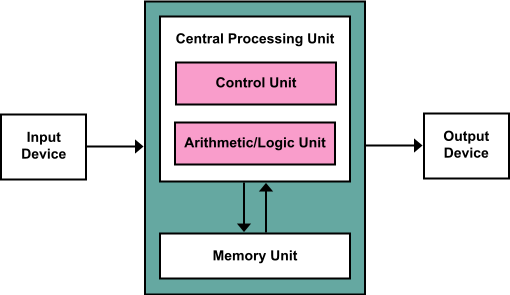
\includegraphics[width=0.75\textwidth]{Figures/VonNewmanArchitecture}
	\\ \parbox{0.75\textwidth}{\caption[VonNewmanArchitecture]{Von Neumann architecture (\url{https://en.wikipedia.org/wiki/Von_Neumann_architecture}) }\label{fig:VonNewmanArchitecture}} 
	\end{figure}
	
	To perform actions, the CPU needs to read from its memory a set of instructions which can be performed under the supervision of the control unit. This set of instructions are called a program, and is written in assembly.
	
	\section{Hardware architecture}\label{theory}
	All of the components are composed of little ON/OFF switches called transistors. In 1965 Gordon E. Moore stated that the number of transistor in a CPU double every year. As a consequence, the machines are more and more complexe and increase their speed each year \footnote{But maybe Moore stated it too fast without thinking on the physic. To avoid quantum effect, it is not possible anymore to reduce the size of the transistor. So we need to adapt our ways of thinking ! \url{http://www.research.ibm.com/ibm-q/learn/what-is-quantum-computing/}}.
	
	\begin{figure}
		\centering
		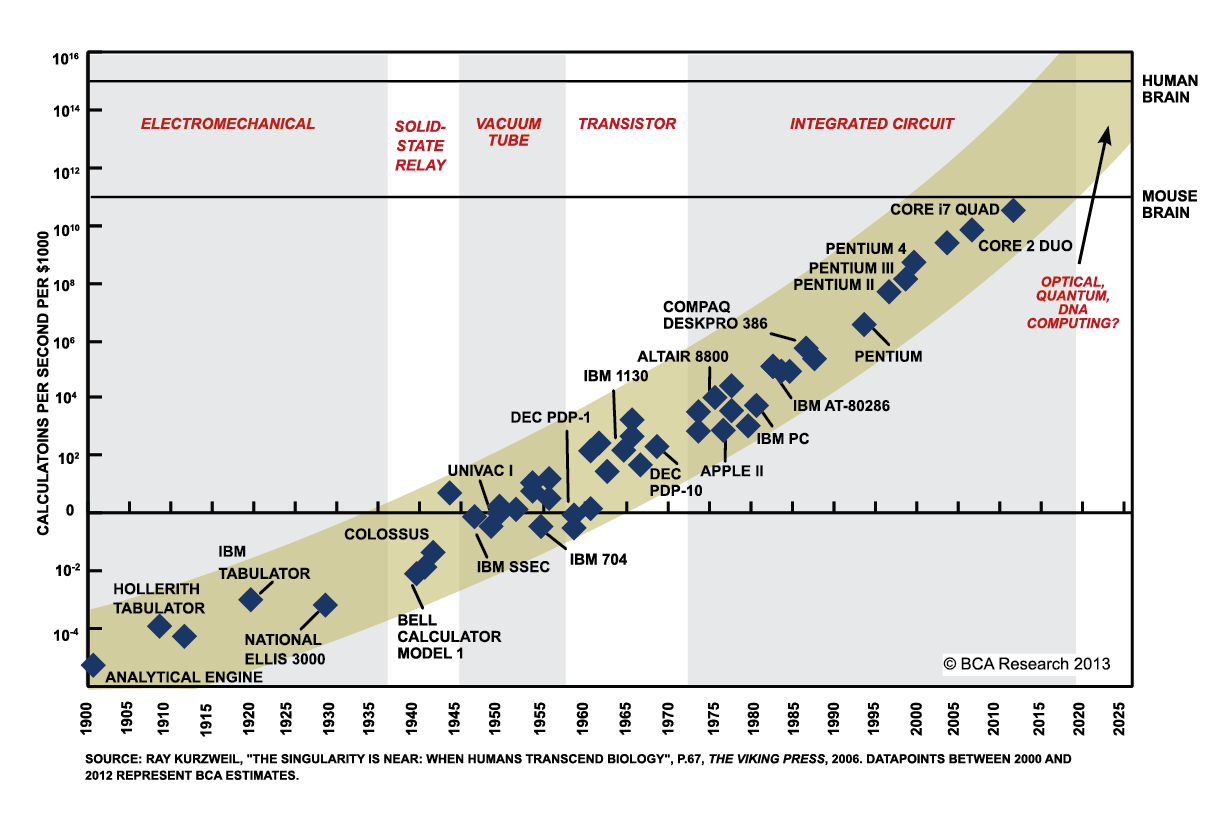
\includegraphics[width=0.75\textwidth]{Figures/MooresLaw2.png}
		\\ \parbox{0.75\textwidth}{\caption[moore]{Moore's law. (\url{https://www.extremetech.com/extreme/210872-extremetech-explains-what-is-moores-law}) }\label{fig:moore}} 
	\end{figure}
	
	\subsection{Memory}
	Two types of memories can be distinguished, the RAM (Random Access Memory) and the ROM (Read-Only Memory).\\ The RAM is intended to store temporary some data, and to have access to it very fast but have not really lot of space. Usually the computer use it when you launch a program, surf the web. Whenever you shut down your computer, the RAM empty itself.
	\\
	The ROM is really slow but provide consistent data, and much more. These can be external or internal drive where you store your pictures, music, program installation...\\
	Usually, the more data you can store, the slower your access will be. Imagine looking for a specific jacket when you have $10$ in your wardrobe, versus when you have $10000$ (and really rich)!
	\subsection{CPU}
	IBM were the first to launch a multi-core processor, the POWER4\cite{tendler2002power4}.
	It consists of multiple "little" CPUs called core. The more core your CPU have, the more thread are available, the more operations can be performed in parallel. Each core usually has one ALU, L1 cache (the fastest memory on your computer) and L2 cache.
	
	\begin{figure}
		\centering
		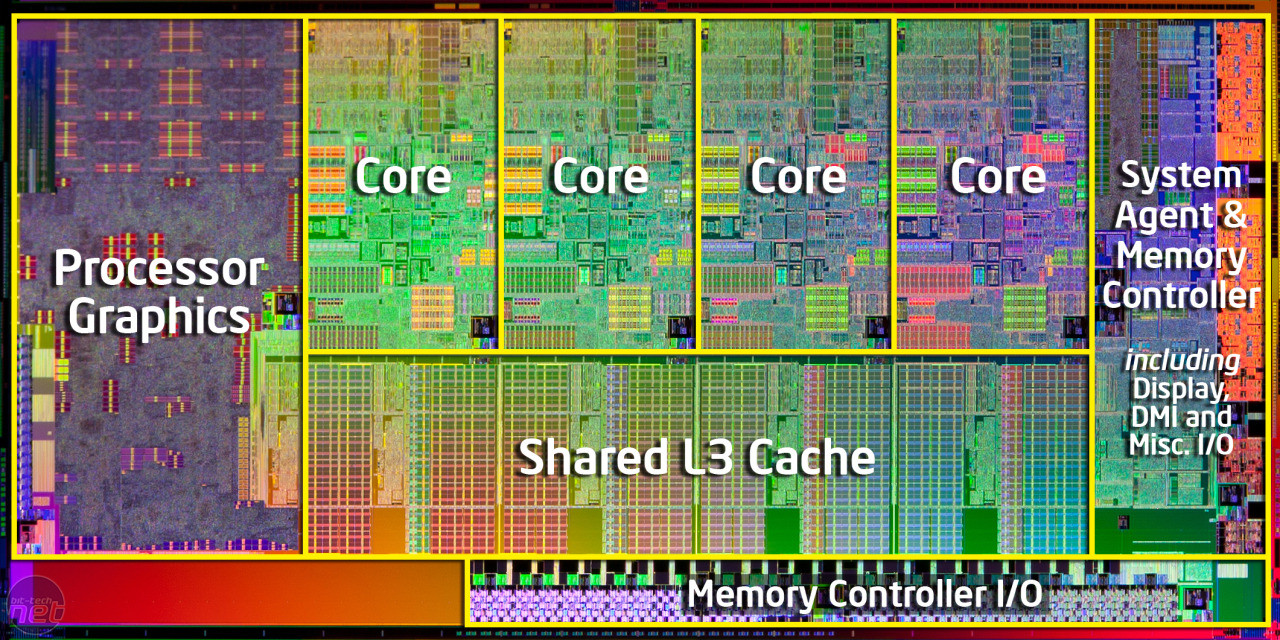
\includegraphics[width=0.75\textwidth]{Figures/multicore}
		\\ \parbox{0.75\textwidth}{\caption[multicore]{Multi-core processor scheme. (\url{https://superuser.com/questions/317936/cpu-core-temperature-variation}) }\label{fig:multicore}} 
	\end{figure}
	
	IGPU (Integrated GPU) will perform basic graphic tasks, it is intended to reduce the load of the GPU (Graphics Processing Unit). It will run for example your graphical OS (Operating System like Windows).\par
	A CPU performs operations which depends on the number of  threads and speed of the clock, if the CPU is synchronous. The clock is the time reference for the component (and all the computer), because it can perform one operations per clock cycle. If you want to perform faster FLOPS (FLoating point Operations Per Second), you need a faster clock.
	\subsection{GPU}
	Read the appropriate article you lazy one !
	\subsection{Alimentation and cooling}
	To provide power to your system, you will need an alimentation. It will convert the AC voltage ($120$ or $240$V) from your house, to  the $12/24$V DC for your PC. Usually $500$ W is enough for a normal computer. If you are aware of your electrical consumption, and want a good quality, look at the certification. For example the certification $80$ PLUS means that your alimentation has an efficiency of minimum $80$\%, $80$ PLUS will have ~$90$\% efficiency.\par
	Cooling is really important because the electronical component produces heat and wear out over time if too hot. Nowadays we have mostly two types of cooling, water cooling or fan cooling. Water cooling is more efficient but more complicated to use and maintain (careful with the leaks and microorganism in the water), fan cooling cost less and easier to use.
	
	\begin{figure}
		\centering
		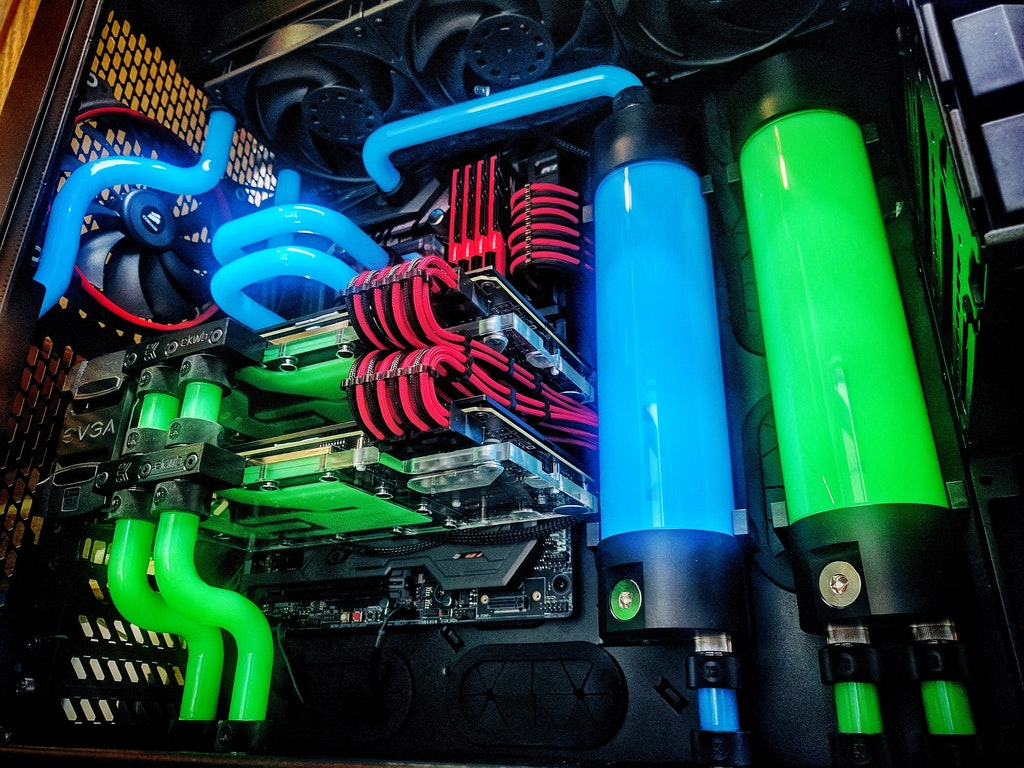
\includegraphics[width=0.75\textwidth]{Figures/watercooling}
		\\ \parbox{0.75\textwidth}{\caption[watercooling]{Example of water cooling system. (\url{https://www.reddit.com/r/watercooling/comments/5yht4l/my_first_watercooling_system/}) }\label{fig:watercooling}} 
	\end{figure}
	
	\subsection{MotherBoard}
	The main board of a computer is used to provide connections between all previously mentioned components. Be careful to choose a motherboard with compatible socket and connectors for your CPU, memory, GPU, fans, audio chip, alim, USB...\\
	Among many connections you have the PCI express which is used to connect your GPU, CPU socket to place your CPU, SATA connectors for external drives, DIMM (Dual Inline Memory Module) for your RAM.
		
	\begin{figure}
		\centering
		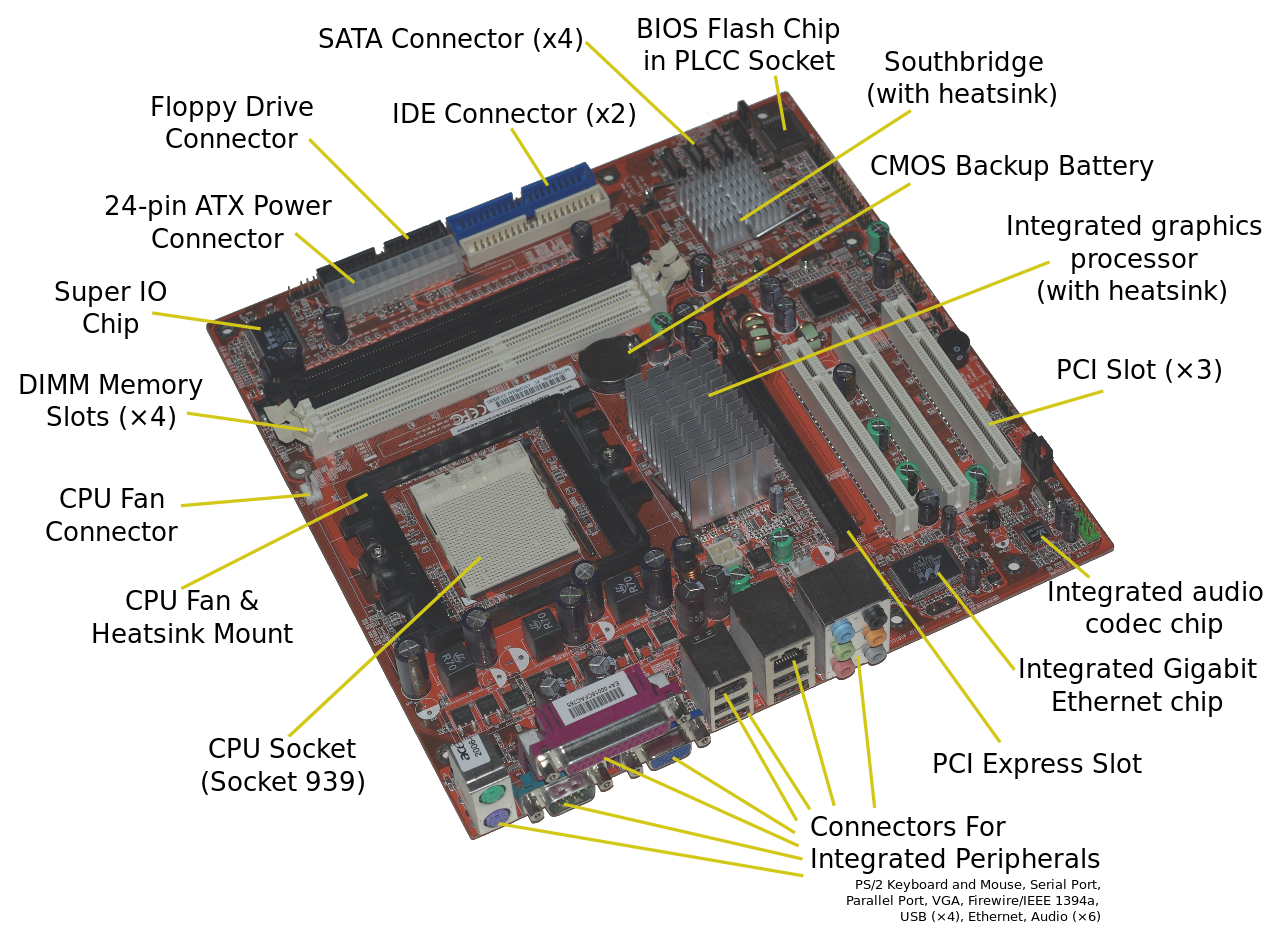
\includegraphics[width=0.75\textwidth]{Figures/MotherBoard}
		\\ \parbox{0.75\textwidth}{\caption[motherboard]{An Acer mother board. (\url{https://en.wikipedia.org/wiki/Motherboard/media/File:Acer_E360_Socket_939_motherboard_by_Foxconn}) }\label{fig:motherboard}} 
	\end{figure}
	
	\section{Assembly language}
	
	Assembly language is the lowest level programming language, where the instructions are directly correlated on the architecture of the device.
	When you compile a program, the compiler will create .asm objects. Theses are set of instruction coded in assembly language, which will later be transformed into binary objects (this is what your CPU understand).\\
	There is a set of low level instructions stored in the processor register unit, but you can also use register to store a specific adress or data. When we are talking about x86 register that's mean that the register is 32bit length (FFFF FFFF), x64 refers to a size of 64bits (FFFF FFFF FFFF FFFF)\footnote{where x refers to the way of stocking variable, in this case little endian.}. For a bus size of $256$ bits, you can process in parallel $8$ x86 instructions.
	
	\begin{figure}
		\centering
		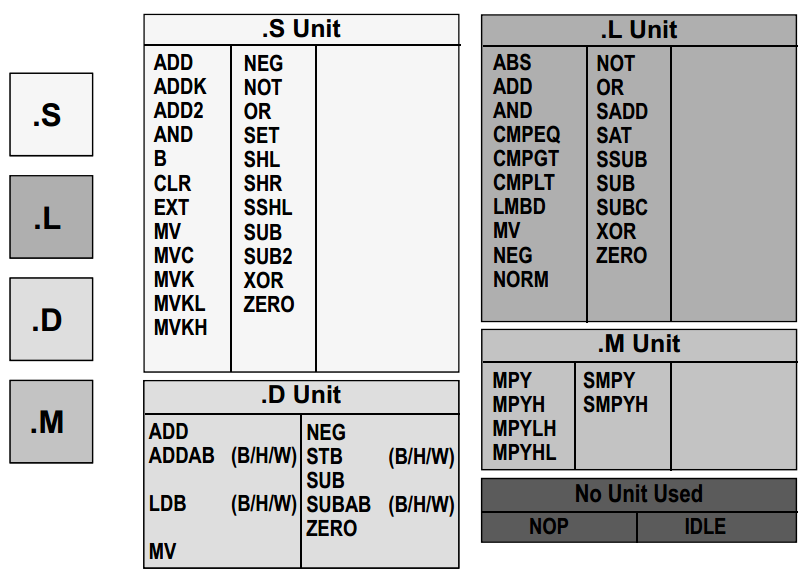
\includegraphics[width=0.75\textwidth]{Figures/registerstable}
		\\ \parbox{0.75\textwidth}{\caption[registerTable]{An example of an instruction set for a DSP C6x. (\url{https://en.wikipedia.org/wiki/Motherboard/media/File:Acer_E360_Socket_939_motherboard_by_Foxconn}) }\label{fig:RegTable}} 
	\end{figure}
	
	\subsection{How to use instructions in assembly ?}
	
	You want to use a datasheet to see how instructions are used,
	for example for DSP...
	.\\.\\.\\.\\.\\
	
	\subsection{Memory Access}
	Here is an example of loading values in asm, where the destinations is on the right, and the source is on the left.
	\begin{lstlisting}[language={[x86masm]Assembler}]
	# A0 = F001
	# A1 = 0000
	LDB A0, A1
	# A1 = 0001
	LDH A0, A1
	# A1 = F001
	STH 2, A1
	# A1 = F002
	\end{lstlisting}
	
	Using pointer is the basic in assembly, you can access to the value stored in a specific adress using operator *. Operators ++, -- are used to increment or decrement and [], () to specify length of step.\par
	[] is used to increment your table by a length specified in your instruction. () allowed you to increment by 1 byte. If you place ++ before the register, it will first increment then operate. For example imagine a memory stored in little endian (x16),
	\begin{lstlisting}[language={[x86masm]Assembler}]
	# in hexadecimal
	LDH 0008, A0
	LDH *A0--[4], A5
	\end{lstlisting}
	will store the value of address A0 in A5, and after decrement the address by 4*16 bit. So the value of A0 is $0x0$,
	Try out to find the others value !
	
	\begin{figure}
		\centering
		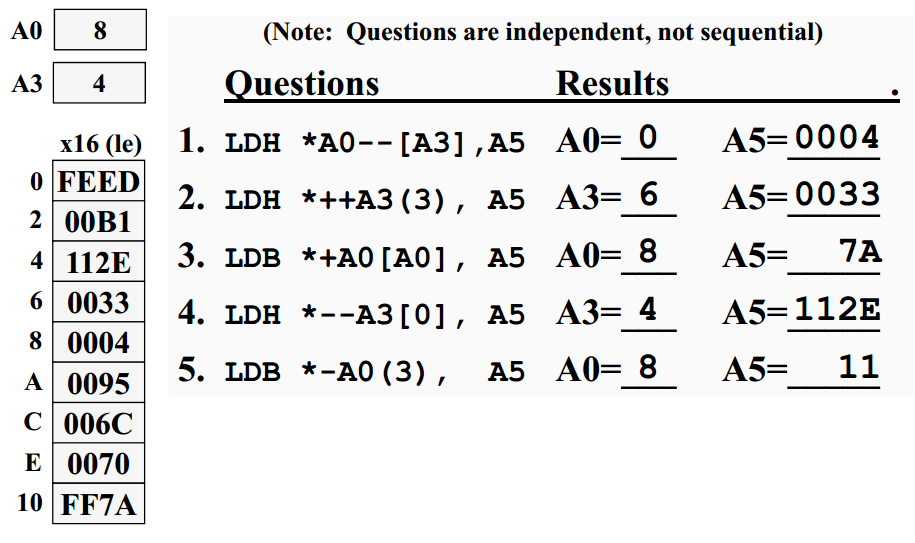
\includegraphics[width=0.75\textwidth]{Figures/examplePointer}
		\\ \parbox{0.75\textwidth}{\caption[examplePointer]{Exercise to understand pointer management in assembly. }\label{fig:examplePointer}} 
	\end{figure}

	\subsection{Conditions and loops}
	.\\.\\.\\.\\.\\
	
	\subsection{Linear assembly vs optimized assembly}
	
	Linear assembly (.sa) is the simplest way to code in assembly language. In contrary to optimized assembly (.asm), you don't need to specify which unit you want to work on (see Fig. \ref{fig:RegTable}). Basically, there is no need to schedule all operations by hand, taking clock cycles into account. With optimized assembly, you can parallelize your code but be careful of the mismatches !
	
	\subsection{Little example of an asm code}
	
	ASM
	
	\begin{lstlisting}[language={[x86masm]Assembler}]
			.global _child2
			.global _w
	_child2: 	MVKL	.S	_w,B0
				MVKH	.S	_w,B0
				MVK		.S	A6,B2
				zero	.L	A1
				
	for:		LDH		.D	*B0++,B1
				LDH		.D	*B4++,B5
				LDH		.D	*A4++,A5
				nop			3
				MPY		.M	B5,B1,B1
				nop
				ADD		.L	A5,B1,B1
				ADD		.L	A1,B1,A1
	[B2]		SUB		.L	B2,1,B2
	[B2]		B		.S	for
				nop			5
				MV		.D	A1,A4
				B		.S	B3
				nop			5			
	
	# A1 = 0000
	LDB A0, A1
	# A1 = 0001
	LDH A0, A1
	# A1 = F001
	STH 2, A1
	# A1 = F002
	\end{lstlisting}
	
	\subsection{Parrallelize and optimize your asm code}
	\label{sec:method}
	http://igoro.com/archive/fast-and-slow-if-statements-branch-prediction-in-modern-processors/
	\section{Conclusion}
	\label{sec:conclusion}
	First of all, I wanted to say that coding some part of a C++ program in assembly is non optimal, since the compiler will often do better than you. It will take lot of time and effort but not so many improvements, it really depend on your application. You need to inspect C/C++ assemblies to see where the compiler is making non-optimal choices.
	ASIIC are another type of "programmation",where you create your own circuits using transistors. So for a typical function you can have verry fast results.
	\subsection*{Acknowledgment}
	Thanks
	
	{\small
		\bibliographystyle{splncs03}
		\bibliography{article}
	}
	
\end{document}

